\chapter{Additions et soustractions de fractions}\label{ChAddSousFrac}

\vspace{5cm}
\begin{acquis}
\begin{itemize}
\item 
\item 
\item 
\end{itemize}
\end{acquis}


\activites  
\begin{activite}[Additions et soustractions]

\begin{partie}[Première partie : Dénominateurs n'ayant pas de diviseur commun autre que 1]

\begin{center}
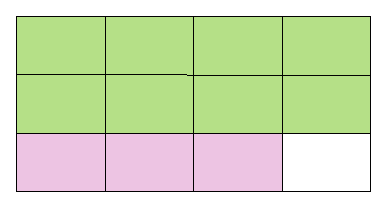
\includegraphics[width=.3\linewidth]{actiADF1}
\end{center}

\begin{enumerate}
\item Complète les phrases suivantes :
    \begin{itemize}
        \item L'aire de la région verte représente $\dfrac{2}{...}$ de l'aire totale ;
        \item L'aire de la région rose représente $\dfrac{1}{...}$ de l'aire totale.
    \end{itemize}
\item \label{ASFacti1} Quel calcul permet d'obtenir l'aire que représente la région coloriée par rapport à l'aire totale ?
\item En t'aidant du dessin, complète l'égalité : $\dfrac{2}{3}+\dfrac{1}{4}=\dfrac{...}{...}$.
\item \label{ASFacti2} Comment retrouver ce résultat par le calcul ?
\end{enumerate}
\end{partie}

\begin{partie}[Deuxième partie : Dénominateurs ayant plusieurs diviseurs communs]
\begin{enumerate}
\item Sur le même rectangle, on veut colorier, en bleu, $\dfrac{1}{8}$ de l'aire et, en orange, $\dfrac{5}{6}$ de l'aire. Quelles dimensions minimales, en nombre entier de centimètres, peux-tu donner à ce rectangle pour que ce partage soit facile à effectuer ? Fais une figure.
\item Reprends les questions \ref{ASFacti1} à \ref{ASFacti2} de la première partie.
\end{enumerate}
\end{partie}

\begin{partie}[Troisième partie : Bilan]
\begin{enumerate}
\item Énonce une règle qui permet d'additionner ou de soustraire des fractions de dénominateurs différents.
\item Applique cette règle pour effectuer les calculs suivants : $\dfrac{1}{5}+\dfrac{7}{2}$ et $\dfrac{7}{10}-\dfrac{11}{15}$.
\end{enumerate}
\end{partie}
\end{activite}





\begin{activite}[Aire d'une portion de disque]

\begin{partie}
\begin{enumerate}
\item Calculer l'aire et le périmètre d'un disque de rayon 9\,cm. On utilisera $\pi \approx 3,14$.
\item Sachant que le rayon mesure 9\,cm, calculer la longueur de l'arc de cercle $AB$ et l'aire du secteur de disque délimité par les rayons $[OA]$ et $[OB]$, et l'arc $AB$, dans chacun des cas suivants :

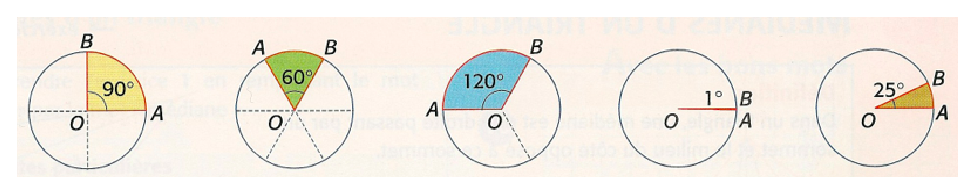
\includegraphics[width=\linewidth]{actiADF2}

\end{enumerate}
\end{partie}

\begin{partie}
L'aire d'un secteur de disque $AOB$ est-elle proportionnelle à la mesure de son angle $\widehat{AOB}$ ? Et la longueur de l'arc $AB$ ?
\end{partie}


\end{activite}


\cours
\section{Réduction de quotients au même dénominateur}

\begin{aconnaitre}
\begin{tabular}{p{.6\linewidth}|p{.35\linewidth}}
Pour additionner ou soustraire des fractions, il faut les mettre au \textbf{même dénominateur}. Pour cela, on utilise la règle suivante : \textbf{Si on multiplie ou si on divise} le numérateur et le dénominateur d'un quotient par \textbf{un même nombre non nul} alors on obtient \textbf{un quotient égal}. & Pour tous nombres $a$, $b$ et $k$ 
où $b$ et $k$ sont non nuls : \[ \dfrac{a\times k}{b \times k} = \dfrac{a}{b} \quad \text{et} \quad \dfrac{a \div k}{b \div k} = \frac{a}{b} \] \\
\end{tabular}
\end{aconnaitre}
 



\begin{exemple*1}

Réduis les quotients $\dfrac{2}{9}$ et $\dfrac{5}{12}$ au même dénominateur.

\correction

\begin{tabular}{lcl}
Multiple de 9 : 9, 18, 27, \textbf{36}, 45, 54,... & &\\
Multiple de 12 : 12, 24, \textbf{36}, 48, 60,... & $\longrightarrow$ & On cherche un multiple commun non nul aux \\
Un multiple commun de 9 et 12 est 36. & & dénominateurs (le plus petit possible). \\
C'est aussi le plus petit. &  &  \\
$\dfrac{2}{9} = \dfrac{2 \times \boldsymbol{4}}{9 \times \boldsymbol{4}} = \dfrac{8}{36}$ et $\dfrac{5}{12} = \dfrac{5\times \boldsymbol{3}}{12 \times \boldsymbol{3}} = \dfrac{15}{36}$ & $\longrightarrow$ & On détermine les écritures fractionnaires ayant \\
& &  36 pour dénominateur. \\
\end{tabular}
\end{exemple*1}


\begin{exemple*1}

Compare les quotients $\dfrac{2}{7}$ et $\dfrac{3}{8}$.

\correction

Les dénominateurs 7 et 8 n'ont aucun diviseur commun autre que 1.

Le plus petit multiple commun est $7 \times  8 = 56$, donc $\dfrac{2 \times \boldsymbol{8}}{7 \times \boldsymbol{8}} = \dfrac{16}{56}$ et $\dfrac{3 \times \boldsymbol{7}}{8 \times \boldsymbol{7}} = \dfrac{21}{56}$.

Rappel : deux fractions qui sont au même dénominateur sont rangées dans le même ordre que leur numérateur : Comme $16 < 21$ alors $\dfrac{16}{56}<\dfrac{21}{56}$ et finalement $\dfrac{2}{7}<\dfrac{3}{8}$.
\end{exemple*1}



\section{Addition ou soustraction}

\begin{aconnaitre}
\begin{tabular}{p{.6\linewidth}|p{.35\linewidth}}
Pour \textbf{additionner (ou soustraire)} des nombres en écriture fractionnaire \textbf{ayant le même dénominateur}, on additionne (ou on soustrait) les numérateurs et on garde le dénominateur commun. & Pour tous nombres $a$, $b$ et $c$ où $b$ est non nul : \[ \dfrac{a}{b}+\dfrac{c}{b}=\dfrac{a+c}{b} \] \\
\end{tabular}
\end{aconnaitre}



\begin{remarque}
Si les nombres en écriture fractionnaire n'ont pas le même dénominateur, il faut les réduire au même dénominateur.
\end{remarque}

\begin{exemple*1}

Calcule l'expression $A =-1+\dfrac{13}{30}-\dfrac{-11}{12}$.

\correction

\begin{tabular}{lcl}
Multiples de 30 : 30 ; \textbf{60} ; 90 ; 120... & & \\
Multiples de 12 : 12 ; 24 ; 36 ; 48 ; \textbf{60}... & $\longrightarrow$ & On cherche le plus petit multiple commun non nul à 30 et 12. \\
$A =\dfrac{-1 \times 60}{1 \times 60}+\dfrac{13 \times 2}{30 \times 2}+\dfrac{11 \times 5}{12 \times 5}$ & $\longrightarrow$ & On détermine le signe de chaque quotient et on réduit les \\
& & quotients au même dénominateur 60. \\
$A =\dfrac{-60}{60}+\dfrac{26}{60}+\dfrac{55}{60}=\dfrac{-60+26+55}{60}$ & $\longrightarrow$ & On additionne les numérateurs et on garde le dénominateur. \\
$A = \dfrac{21}{60}=\dfrac{7 \times 3}{20 \times 3}= \dfrac{7}{20}$ & $\longrightarrow$ & On simplifie si possible. \\
\end{tabular}

\end{exemple*1}





\exercicesbase
\begin{colonne*exercice}
\serie{Comparaison}

\begin{exercice}[Signes]

Donne le signe des nombres suivants :
$\dfrac{-5,2}{4,23}$ ; $\dfrac{5}{-2,1}$ ; $\dfrac{472}{23}$ ; $\dfrac{-8,9}{-45}$ ; $-\dfrac{12}{13}$ ; $-\dfrac{11}{-5,2}$.
\end{exercice}

\begin{exercice}

Indique les nombres égaux parmi ceux de la liste ci-dessous :
$\dfrac{-8}{9}$ ; $-\dfrac{8}{9}$ ; $\dfrac{-8}{-9}$ ; $-\dfrac{8}{-9}$ ; $\dfrac{8}{-9}$ ; $-\dfrac{-8}{9}$ ; $\dfrac{8}{9}$.
\end{exercice}

\begin{exercice}[Encadrement]

\begin{colenumerate}{1} 
\item On considère la fraction $\dfrac{56}{21}$.

Effectue la division euclidienne de 56 par 21 et déduis-en un encadrement de la fraction par deux nombres entiers consécutifs.
\item Encadre $\dfrac{-89}{15}$ puis $\dfrac{47}{59}$ par deux nombres entiers consécutifs.
\item Encadre respectivement $\dfrac{-47}{25}$ et $\dfrac{13}{-4}$ par deux nombres entiers consécutifs et déduis-en la comparaison de ces deux fractions.
\item Peux-tu appliquer la même méthode pour comparer $\dfrac{25}{3}$ et $\dfrac{90}{11}$ ?
\end{colenumerate} 
 
\end{exercice}

\begin{exercice}[Avec des valeurs approchées]
Soient deux nombres : $a = \dfrac{816}{577}$ et $b = \dfrac{577}{408}$.

\begin{colenumerate}{1} 
\item Donne la valeur arrondie de $a$ et celle de $b$ au millième. Peux-tu en déduire la comparaison de $a$ et de $b$ ?
\item Donne des valeurs approchées de $a$ et $b$ qui permettent de les comparer. Compare $a$ et $b$.
\end{colenumerate} 
 
\end{exercice}

\begin{exercice}[Égalités]

Recopie et complète chacune des égalités suivantes :

\begin{colenumerate}{2} 
\item $\dfrac{...}{-5} = \dfrac{10}{20}$
\item $\dfrac{2}{3} = \dfrac{...}{27}$
\item $\dfrac{-15}{45} = \dfrac{-5}{...}$
\item $\dfrac{...}{-18} = \dfrac{7}{6}$
\item $3 = \dfrac{...}{4}$
\item $-2,1 = -\dfrac{21}{...}$
\end{colenumerate} 
 
\end{exercice}

\begin{exercice}

Dans chaque cas, à partir des égalités données et en utilisant seulement les quatre nombres qui apparaissent, écris toutes les égalités d'écritures fractionnaires possibles :

\begin{colenumerate}{2} 
\item $7 \times (-8) = -4 \times 14$
\item $-3 \times (-1) = 2 \times 1,5$
\item $2,1 \times 12 = 9 \times 2,8$
\item $-4 \times 9 = 12 \times (-3)$
\end{colenumerate} 
 
\end{exercice}

\begin{exercice}[Égalité ?]
Recopie et complète en utilisant = ou $\neq$, en justifiant dans chaque cas :

\begin{colenumerate}{1} 
\item $\dfrac{-9,1}{5,2} \quad ... \quad \dfrac{79,8}{-45,6}$ 
\item $\dfrac{-5}{-3} \quad ... \quad \dfrac{-3,5}{2,1}$
\item $\dfrac{17,36}{-22,32} \quad ... \quad -\dfrac{28,7}{36,9}$
\item $\dfrac{-56}{-57} \quad ... \quad \dfrac{57}{58}$
\end{colenumerate} 
\end{exercice}


\begin{exercice}[Avec un dénominateur entier positif]

Réécris chacune des écritures fractionnaires suivantes avec un dénominateur entier positif :
$\dfrac{4}{-5}$ ; $\dfrac{-8}{-7}$ ; $-\dfrac{5,2}{-7}$ ; $\dfrac{7}{-2,1}$ ; $\dfrac{8,2}{0,12}$ ; $-\dfrac{-1}{-3,54}$.
\end{exercice}



\begin{exercice}[Même dénominateur positif]

\begin{colenumerate}{1} 
\item Recopie et complète la phrase suivante :

\og Deux nombres en écriture fractionnaire de même dénominateur positif sont rangés... \fg.
\item Compare les nombres suivants :

$\dfrac{-7,5}{3} \text{ et } \dfrac{-7,49}{3}$

$\dfrac{4,05}{2,1} \text{ et } \dfrac{4,2}{2,1}$

$-\dfrac{0,74}{5} \text{ et } \dfrac{-0,7309}{5}$

$\dfrac{8}{-5,23} \text{ et } \dfrac{-7,9}{5,23}$
\end{colenumerate} 
\end{exercice}

\begin{exercice}[Avec le même numérateur]

\begin{colenumerate}{1} 
\item Recopie et complète la phrase suivante :

\og Deux nombres positifs en écriture fractionnaire de même numérateur sont rangés... \fg
\item Compare les nombres suivants :

$\dfrac{3,5}{8,2} \text{ et } \dfrac{3,5}{8,15}$

$-\dfrac{-1}{6} \text{ et } \dfrac{1}{5,7}$
\end{colenumerate} 
\end{exercice}

\begin{exercice}[Avec le même numérateur (bis)]

Compare les nombres suivants en commençant par comparer leurs opposés :

\begin{colenumerate}{2} 
\item $\dfrac{1}{-5}$ et $\dfrac{1}{-7}$
\item $\dfrac{-3}{8}$ et $\dfrac{-3}{8,2}$
\item $-\dfrac{5,23}{14,5}$ et $\dfrac{-5,23}{14,6}$
\item $\dfrac{-7,5}{0,23}$ et $\dfrac{75}{-2,4}$
\end{colenumerate} 
\end{exercice}




\begin{exercice}

Dans chaque cas, réécris les nombres avec le même dénominateur positif puis compare-les :

\begin{colenumerate}{2} 
\item $\dfrac{-5}{4}$ et $\dfrac{-9}{8}$ 
\item $\dfrac{2,7}{-9}$ et $\dfrac{-1}{3}$ 
\item 3 et $-\dfrac{20,9}{-7}$ 
\item $-\dfrac{2}{11}$ et $\dfrac{-5}{33}$ 
\item $\dfrac{7}{2,5}$ et $\dfrac{20,5}{7,5}$ 
\item $\dfrac{13}{-27}$ et $\dfrac{-79}{162}$
\end{colenumerate} 
\end{exercice}

\begin{exercice}[Multiple commun]

\begin{colenumerate}{1} 
\item Quels sont les dix premiers multiples de 12 ? Ceux de 18 ? Déduis-en le plus petit multiple non nul commun à 12 et 18, puis un dénominateur commun positif des fractions :

\[ \dfrac{-7}{12} \quad \text{et} \quad \dfrac{-11}{18} \]

Compare alors ces deux nombres.

\item La méthode précédente permet-elle de trouver rapidement un dénominateur commun aux nombres :
\[ \dfrac{8}{11} \quad \text{et} \quad \dfrac{10}{13} \quad \text{?} \]

Comment en trouver un alors rapidement ? Compare ces deux nombres.
\end{colenumerate} 
\end{exercice}

\begin{exercice}

Dans chaque cas, réécris les nombres avec le même dénominateur positif, puis compare-les :

\begin{colenumerate}{2}
\item $\dfrac{-5}{8}$ et $\dfrac{-3,8}{6}$ 
\item $\dfrac{14}{5}$ et $\dfrac{20}{7}$ 
\item $\dfrac{3}{-50}$ et $-\dfrac{4}{75}$ 
\item $\dfrac{54,5}{0,27}$ et $\dfrac{-2,62}{-0,13}$
\end{colenumerate} 
\end{exercice}

\begin{exercice}

Compare en justifiant :

\begin{colenumerate}{2} 
\item $-\dfrac{12}{18}$ et $\dfrac{399}{-300}$ 
\item $\dfrac{2}{57}$ et $\dfrac{1}{28,4}$ 
\item $\dfrac{-75}{11}$ et $\dfrac{31}{-15}$ 
\item $\dfrac{-5}{6}$ et $-\dfrac{15}{14}$ 
\item $\dfrac{6}{13}$ et $\dfrac{29}{65}$ 
\item $\dfrac{-3}{22}$ et $\dfrac{4,5}{33}$
\end{colenumerate} 
\end{exercice}

\begin{exercice}[Dans l'ordre]

\begin{colenumerate}{1} 
\item Range les nombres suivants dans l'ordre croissant sans utiliser de valeurs approchées :
\[ \dfrac{7}{-15} ; \dfrac{7}{3} ; \dfrac{490}{420} ; \dfrac{-5}{12} ; \dfrac{-24}{-18} ; 2,5\]
\item Range les nombres suivants dans l'ordre décroissant
\[ \dfrac{-29}{100} ; \dfrac{7}{-25} ; -0,285 ; -\dfrac{1}{5} ; \dfrac{13}{-50} ; 0 ; \dfrac{-1}{2,5} \]
\end{colenumerate} 
\end{exercice}

\begin{exercice}[Trajet]
Quatre amis font un voyage en trois jours. Le premier jour, ils parcourent 40\,\%\ du trajet total ; le deuxième jour, un quart et le dernier jour, $\dfrac{7}{20}$ du trajet total.

Quel jour ont-ils parcouru la plus grande distance ?

Peux-tu calculer la distance parcourue chaque jour ?
\end{exercice}




\serie{Additions, soustractions}



\begin{exercice}[La règle]
Calcule les sommes et les différences suivantes en respectant les étapes :
\[ \dfrac{-4}{5} + \dfrac{7}{5} = \dfrac{... + ...}{...} = \dfrac{...}{...} \]

\begin{colenumerate}{2} 
\item $\dfrac{9}{7} + \dfrac{-8}{7}$
\item $\dfrac{5,2}{41} + \dfrac{8,56}{41}$
\item $\dfrac{-5}{3} + \dfrac{-6}{3}$
\item $-\dfrac{7}{15} - \dfrac{7}{15}$
\item $\dfrac{56}{57} - \dfrac{58}{57}$
\item $\dfrac{-1}{3} - \dfrac{2}{3}$
\item $\dfrac{-5}{14} - \dfrac{-2}{14}$
\item $\dfrac{1}{8} - \dfrac{9}{8}$
\item $\dfrac{5}{12} + \dfrac{11}{12} - \dfrac{7}{12}$
\item $-\dfrac{1}{25} - \dfrac{-11}{25} + \dfrac{-8}{25}$
\end{colenumerate} 
\end{exercice}

\begin{exercice}[Dénominateurs positifs]

Calcule en réécrivant dans chaque cas les fractions avec le même dénominateur positif :

\begin{colenumerate}{2} 
\item $\dfrac{8}{-5} + \dfrac{7}{5}$
\item $\dfrac{-4}{-15} + \dfrac{1}{-15}$
\item $\dfrac{5}{6} - \dfrac{7}{-6}$
\item $\dfrac{-9}{17} + \dfrac{1}{-17}$
\end{colenumerate} 
 

\end{exercice}

\begin{exercice}[Même dénominateur]
Écris les nombres suivants, si c'est possible, sous la forme $\dfrac{a}{30}$, où $a$ est un nombre décimal relatif :
\[ \dfrac{3}{10} ; \dfrac{1}{-3} ; -2 ; \dfrac{2,1}{0,6} ; \dfrac{-18}{90} ; \dfrac{1}{7} ; \dfrac{1}{-60} \]
\end{exercice}

\begin{exercice}[Avec un multiple]

\begin{colenumerate}{1} 
\item On remarque que $3 \times 8 = 24$ ;

Calcule : $\dfrac{-5}{24}+\dfrac{1}{3}$ en écrivant les fractions avec le même dénominateur positif.

\item Combien de quart(s) faut-il pour faire une unité ? Calcule $1 - \dfrac{5}{4}$ en écrivant les fractions avec le même dénominateur positif.
\item Complète : $-3 = \dfrac{...}{1} = \dfrac{... \times ...}{1 \times ...} = \dfrac{...}{8}$ .
Calcule $-3 + \dfrac{5}{-8}$ en écrivant les fractions avec le même dénominateur positif.
\end{colenumerate} 
\end{exercice}




\begin{exercice}

Effectue les calculs suivants en détaillant les étapes :

\begin{colenumerate}{2} 
\item $\dfrac{5}{6} + \dfrac{-1}{3}$
\item $\dfrac{7}{9} - \dfrac{1}{-27}$
\item $-\dfrac{8}{5} + \dfrac{23}{50}$
\item $\dfrac{45}{15} - \dfrac{7}{3}$
\item $\dfrac{4}{11} + 2$
\item $\dfrac{8}{-91} + \dfrac{-1}{7}$
\item $\dfrac{5}{2} - \dfrac{-45}{4} + \dfrac{2}{8}$
\item $4 - \dfrac{5}{-49} + \left(-\dfrac{8}{7}\right)$
\end{colenumerate}
\end{exercice}

\begin{exercice}[Trouver un dénominateur commun]

\begin{colenumerate}{1} 
\item Écris la liste des premiers multiples de 8 puis celle des premiers multiples de 6. Trouve le plus petit multiple non nul commun à 8 et 6.
 
Utilise alors ce nombre pour écrire les fractions $\dfrac{-5}{7}$ et $\dfrac{7}{6}$ avec le même dénominateur positif et calcule : $\dfrac{-5}{7}+\dfrac{7}{6}$.
\item Cette méthode permet-elle de trouver rapidement un dénominateur commun pour calculer : $\dfrac{5}{17}+\dfrac{1}{50}$ ?

Quel dénominateur commun choisir alors ? Calcule cette somme.
\end{colenumerate} 
\end{exercice}



\begin{exercice}

Effectue les calculs suivants en détaillant les étapes :

\begin{colenumerate}{2} 
\item $\dfrac{-7}{50} + \dfrac{2}{75}$
\item $\dfrac{1}{5} + \dfrac{-2}{3}$
\item $\dfrac{1}{12} - \dfrac{1}{9}$
\item $\dfrac{4}{18} + \dfrac{5}{27}$
\item $\dfrac{17}{-24} + \left(-\dfrac{5}{36}\right)$
\item $\dfrac{3}{16} - \dfrac{-1}{12}$
\item $\dfrac{8}{-17} - \left(-\dfrac{1}{15}\right)$
\item $\dfrac{2}{5} + \dfrac{-2}{15} - \dfrac{7}{12}$
\end{colenumerate} 
\end{exercice}

\begin{exercice}

Effectue les calculs suivants en détaillant les étapes et donne les résultats sous la forme d'une fraction irréductible :

\begin{colenumerate}{2} 
\item $\dfrac{42}{75} - \left(-\dfrac{22}{30}\right)$
\item $\dfrac{85}{4} + \dfrac{25}{-5}$
\item $\dfrac{-12}{25} -8$
\item $-\dfrac{14}{27} + \dfrac{-5}{108}$
\item $\dfrac{9}{-55} - \dfrac{-7}{44}$
\item $\dfrac{-9}{-18} - \dfrac{5}{30} + \left(-\dfrac{9}{6}\right)$
\item $\dfrac{1}{15} + \left(-\dfrac{1}{18}\right)$
\item $\dfrac{3}{-7} + \dfrac{2}{5}-\dfrac{4}{3}$
\end{colenumerate} 
 
\end{exercice}



\begin{exercice}[Héritage]
Après de longues négociations, il a été convenu que Léa héritera de deux quinzièmes de la fortune de son oncle du bout du monde ; Florian, d'un neuvième de cette fortune ; Jean et Justine se partageront équitablement le reste.

Quelles seront les parts respectives de Jean et Justine ?
\end{exercice}

\begin{exercice}[Opposés] 
Complète les égalités suivantes et écris, dans chaque cas, trois phrases utilisant le mot \og opposé(s) \fg :

\begin{colenumerate}{2} 
\item $\dfrac{-2}{5} + ... =0$
\item $... + \dfrac{7}{-8} = 0$
\item $... + \dfrac{-12}{-8} = 0$
\item $\left(-\dfrac{4}{5}\right) + \dfrac{9,6}{12} = ...$
\end{colenumerate} 
\end{exercice}



\begin{exercice}[Avec des lettres]
On donne : $a = \dfrac{-8}{28}$ ; $b = \dfrac{1}{35}$ et $c = \dfrac{45}{-21}$.

\begin{colenumerate}{1} 
\item Calculer $a - b + c$ et $b - a - c$.
\item Que remarques-tu ?
\end{colenumerate} 
\end{exercice}




\serie{Des équations avec des fractions}





\begin{exercice}

Résous les équations suivantes :

\begin{colenumerate}{2} 
\item $x - \dfrac{5}{4} = \dfrac{4}{3}$
\item $x + \dfrac{7}{3} = \dfrac{5}{7}$
\item $x - \dfrac{5}{8} = \dfrac{3}{12}$
\item $\dfrac{1}{3} - x = -\dfrac{2}{9}$
\item $\dfrac{5}{18} - x = \dfrac{11}{45}$
\item $x - \dfrac{12}{25} = -\dfrac{11}{15}$
\end{colenumerate} 
\end{exercice}

\begin{exercice}[Équations du type $ax = b$]

Résous les équations suivantes :

\begin{colenumerate}{3} 
\item $\dfrac{x}{5} = \dfrac{3}{4}$
\item $\dfrac{x}{7} = \dfrac{7}{6}$
\item $\dfrac{x}{11} = -\dfrac{2}{13}$
\item $\dfrac{x}{-8} = \dfrac{8}{9}$
\item $-\dfrac{x}{12} = \dfrac{7}{3}$
\item $\dfrac{7x}{2} = \dfrac{1}{4}$
\item $\dfrac{2x}{9} = -\dfrac{7}{27}$
\item $\dfrac{-3x}{7} = \dfrac{7}{8}$
\item $\dfrac{-11}{9}x = \dfrac{-1}{5}$
\end{colenumerate} 
\end{exercice}

\begin{exercice}[Équations du type $ax + b = c$]

Résous les équations suivantes :

\begin{colenumerate}{2} 
\item $\dfrac{7}{9} y + 5 = 8$
\item $\dfrac{1}{16} x - 2 = \dfrac{5}{8}$
\item $\dfrac{1}{4} x - \dfrac{3}{8} = \dfrac{2}{3}$
\item $\dfrac{3}{7} y - \dfrac{5}{35} = -\dfrac{8}{14}$
\end{colenumerate} 
\end{exercice}

\begin{exercice}

Résous les équations suivantes :

\begin{colenumerate}{2} 
\item $\dfrac{X}{3} = \dfrac{x}{4} - \dfrac{6}{5}$
\item $\dfrac{5x}{8} - \dfrac{3}{10} = \dfrac{7x}{40}$
\item $\dfrac{2x}{7} + \dfrac{3}{14} = \dfrac{x}{7} - \dfrac{1}{14}$
\item $\dfrac{2}{5} x - \dfrac{1}{9} = \dfrac{3}{9} x + \dfrac{4}{5}$
\end{colenumerate} 
\end{exercice}






\serie{Problèmes avec fractions}




\begin{exercice}[Impôts sur le revenu]
Le calcul de l'impôt $I$ pour un revenu annuel imposable $R$ (abattement des 10\,\%\ inclus) compris entre 11 198 € et 24 872 € est basé sur la relation suivante : $I =\dfrac{14}{100}R - 857$. 
Quel est le revenu annuel imposable $R$ d'un individu qui paie 1 040 € d'impôts ?
\end{exercice}



\begin{exercice}

Trouve une fraction égale à $\dfrac{4}{3}$ dont la somme du numérateur et du dénominateur est égale à 63 (tu appelleras $x$ le numérateur de la fraction recherchée). 
\end{exercice}



\begin{exercice}[Un rectangle...]

Les longueurs sont données en cm et les aires en cm$^2$.

$L$ et $\ell$ désignent respectivement la longueur et la largeur d'un rectangle. On sait que l'aire de ce rectangle est de 230,4 et que $\dfrac{L}{\ell}=\dfrac{5}{2}$.

\begin{colenumerate}{1} 
\item Calculer les mesures exactes de la longueur et de la largeur de ce rectangle.
\item Calculer la mesure exacte du périmètre de ce rectangle.
\end{colenumerate} 
\end{exercice}



\begin{exercice}[Drôle de nombre]
Si on retranche un même nombre au numérateur et au dénominateur de la fraction $\dfrac{4}{5}$, on obtient la fraction $\dfrac{5}{4}$.

Trouver ce nombre.
\end{exercice}

\end{colonne*exercice}


%\exercicesappr
%\begin{colonne*exercice}
%\input{AddSousFrac/AddSousFrac_exos_approf}
%\end{colonne*exercice}

\connaissances
%\input{AddSousFrac/AddSousFrac_qcm.tex}

%\TravauxPratiques
%\input{AddSousFrac/AddSousFrac_enGrp.tex}

\Recreation % avec R majuscule pour saut de page
%\input{AddSousFrac/AddSousFrac_finChap.tex}


